
\chapter{Systemarkitektur}
\begin{longtabu} to \linewidth{@{}l l l X[l]@{}}
	
	
	Version &    Dato &    Ansvarlig &    Beskrivelse\\[-1ex]
	\midrule
	0.1 &    03-11-2015 &    MB &    Oprettelse \\[-1ex]
	0.2 &    10-11-2015 &    DHC, MB &    Start af skrivning, indsætning af billeder Hardware  \\[-1ex]
	0.3 &  11-11-2015   &  DHC   &   Forstrækning  \\[-1ex]
	
	\label{version_Systemark}
\end{longtabu}

I det følgende beskrives arkitekturen for systemet. Systemarkitekturen er vores udviklingsramme for den videre udvikling af design og implementering af blodtrykssystemet. Designet af systemet er grebet an således at først kigges der på det overordnede system, hvorefter systemet arbejdes ned i mindre brudstykker. Dette gøres ved at benytte diagrammer med tilhørende beskrivelser.

\section{Hardware}
\subsection{Design}

Systemets hardware kan illustreres i et BBD. Det ses at nedestående figur at systemet består af fem hardware blokke: software system, forstærker, filter, DAQ og transducer. Disse fem blokke udgør til sammen selve blodtryksmåleren.  
	
\begin{figure}[htb]
	\centering
	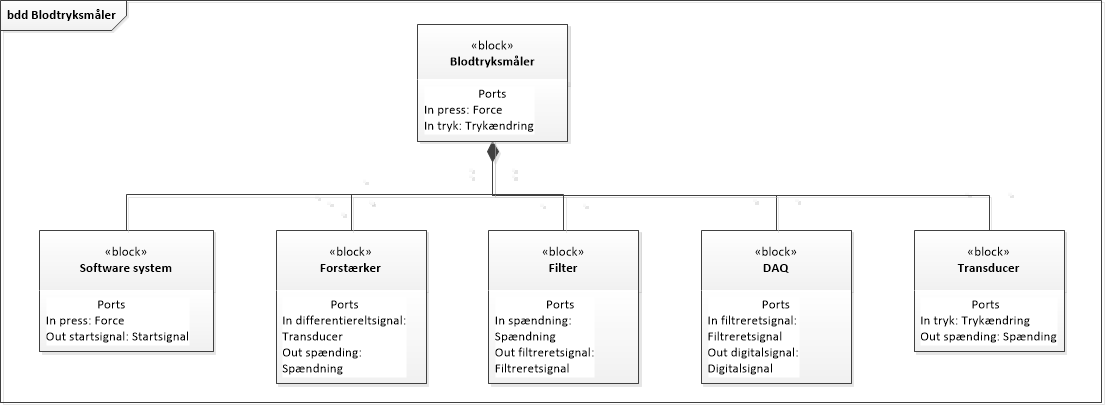
\includegraphics[width=1.0\textwidth]{Figurer/BDD}
	\caption{Block Definition Diagram for hardware}
	%\label{fig:BDD viser blodtrykssystemets hardwaredele, samt sammenhængen mellem disse}
\end{figure}

Ovenstående BDD-diagram fører videre til udarbejdelsen af IBD for hardware komponenterne. I dette diagram vises koblingen mellem de forskellige blokke gennem port forbindelser.  Det ses at signalet starter ved transduceren, hvorefter det bliver behandlet gennem forstærker, filter og DAQ. Til sidste sendes det ind i software systemet, som bliver påvirket at tryk på knapper på GUI. 

\begin{figure}[htb]
	\centering
	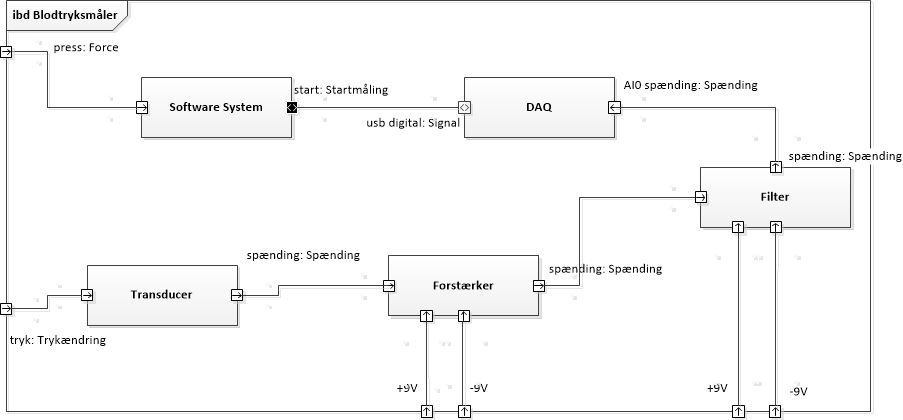
\includegraphics[width=1.0\textwidth]{Figurer/IBD}
	\caption{Infernal Block Diagram for hardware}
	\label{fig:IBD viser koblingen mellem blodtrykssystemets hardwaredele}
\end{figure}

\subsubsection{Forstærkning}
Transduceren måler en trykændring som den omsætter til en spænding. Dette er udtrykt ved et differentieret signal, som sendes ind i forstærkning-blokken. Da signalet fra transduceren ligger i et interval på 0 - 11.28 mV,  skal dette forstærkes op så det passer med NI-DAQ. I projektet er det valgt at DAQ'ens input skal ligge mellem 0-5V. Derved skal signalet forstærkes: 
\begin{equation}
11.28mV\cdot x = 5 V \Rightarrow x= 443
\end{equation}
Under simulering bruges Analog Discovery som en funktionsgenerator, der simulere det differentieret signal. Analog Discovery har dog en vis usikkerhed, når der arbejdes med små spændinger. Dette kan modarbejdes med en spændingsdeler, hvor der bygges et kredsløb som ligger før selve forstærkningen. Dette gør at Analog Discovery kan sende en højere spænding, som så gøre mindre igen ved spændingsdeler princippet.  

\subsubsection{Lavpas}
I projektet skal der laves et 2. ordens lavpasfilter. Dette filter skal være et Salen-Key Buttenworth-filter, med en knækfrekvens på 50 Hz. 

\subsection{Implementering}
\subsubsection{Forstærkning}
For at få den rette forstærkning har vi valgt at benytte operationsforstærkeren INA-114. Her kan transduceren sættes på med det differentieret signal. Under opbygning og modultestning vil det differentieret signal blive simuleret af Analog Discovery.
For at få den rette forstærkning ændres der på den "indre" modstand ($ R_g $) til INA114.
 
For at imøde usikkerheden ved Analog Discovery, laves et lille kredsløb efter spændingsdeler princippet. Her bruges $ R_1=10k\Omega $ og $ R_2 = 1k\Omega $. Da vi kender det signal som skal ind i INA-114 og modstanden kan vi derved finde størrelsen af den spænding som skal sende fra Analog Discovery.
 
\begin{equation}
U_{INA} = U_{analog} \cdot \frac{R_2}{R_1 + R_2} \Rightarrow 5mV = U_{analog}\cdot \frac{R_2}{R_1+R_2} \Rightarrow U_{analog}= 55mV
\end{equation} 

\subsubsection{Lavpas}
For at opnå den ønskede effekt i lavpasfilteret, blev det oplyst at $ f_c=50$ Hz, $ R_1 = R_2 $ og $ C_2=680 nF$. Ud fra det udregnes de resterende komponentværdier for filteret.  


\subsection{Modultest}
\subsubsection{Forstærkning}
\subsubsection{Lavpas}
For at teste lavpasfilteret foretages målinger med en sinus, hvor frekvensen variere for hver måling. Derved aflæses fasen, mellem indgang- og udgangssignal, og amplituden for hver måling. 
Ved knækfrekvensen skal fasendrejningen være 90\textdegree. Amplituden skal ændre sig XXX. Dette kan aflæses på billedet Måling for 50 Hz.
Efter knækfrekvensen skal amplituden blive mindre og mindre(går mod nul). På Måling for 60 Hz, kan det ses hvordan amplituden er faldet drastisk efter knækfrekvensen.  \\
\begin{figure}[htb]
	\centering
	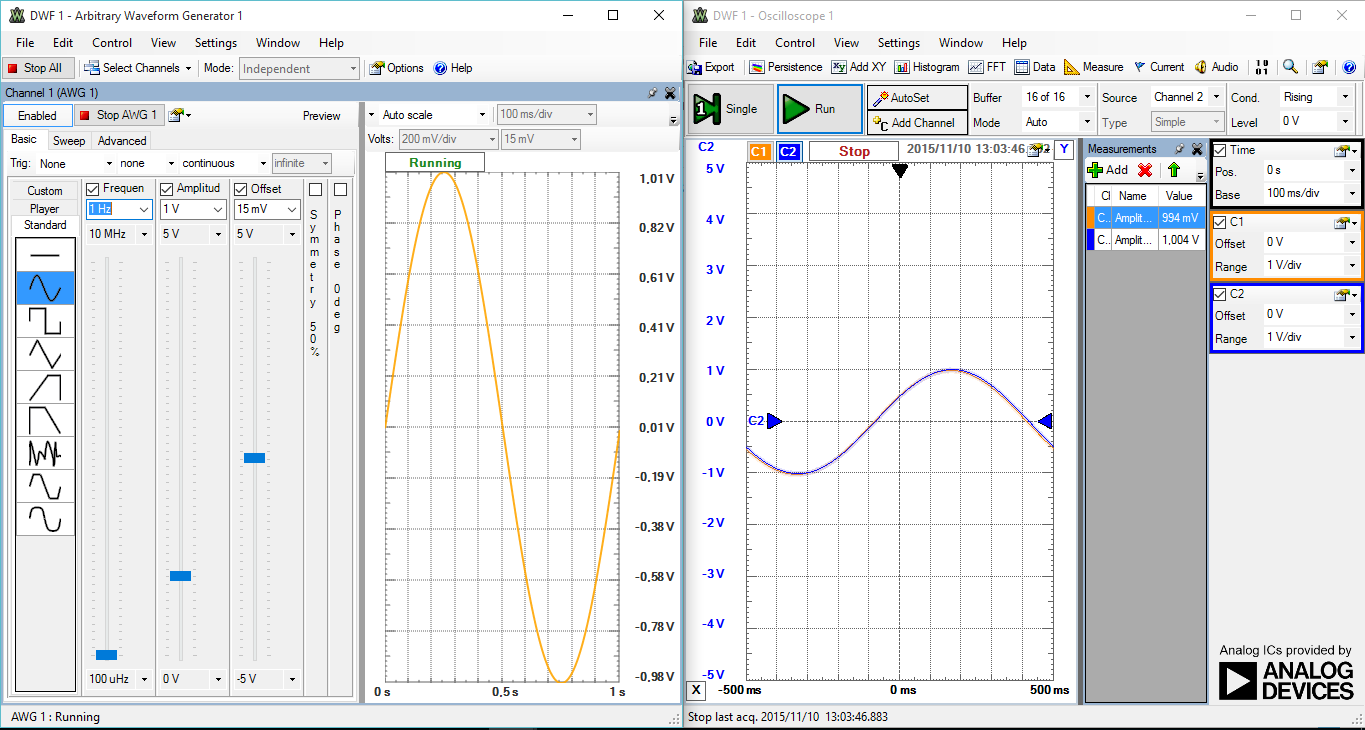
\includegraphics[width=1.0\textwidth]{Figurer/10Hz}
	\caption{Måling for 10 Hz}
	\label{fig:maeling10Hz}
\end{figure}

\begin{figure}[htb]
	\centering
	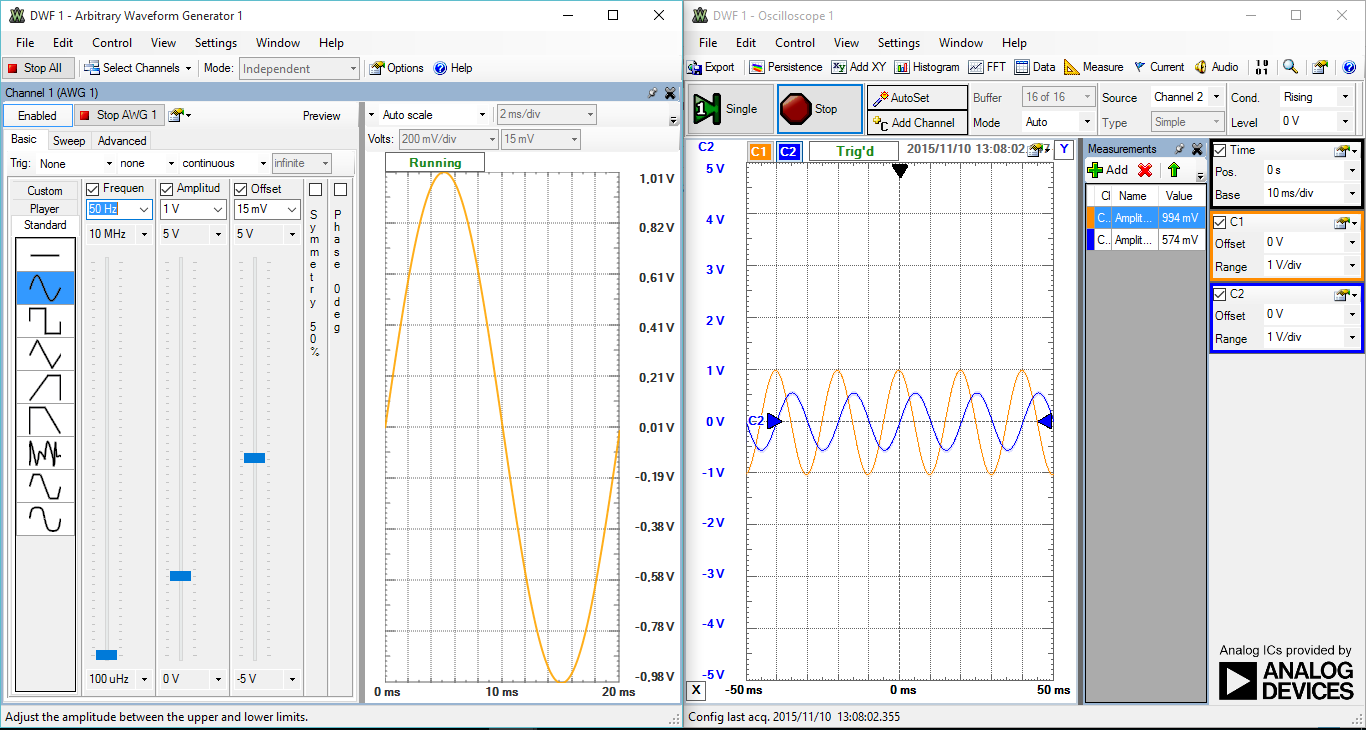
\includegraphics[width=1.0\textwidth]{Figurer/50Hz}
	\caption{Måling for 50 Hz}
	\label{fig:maeling50Hz}
\end{figure}

\begin{figure}[htb]
	\centering
	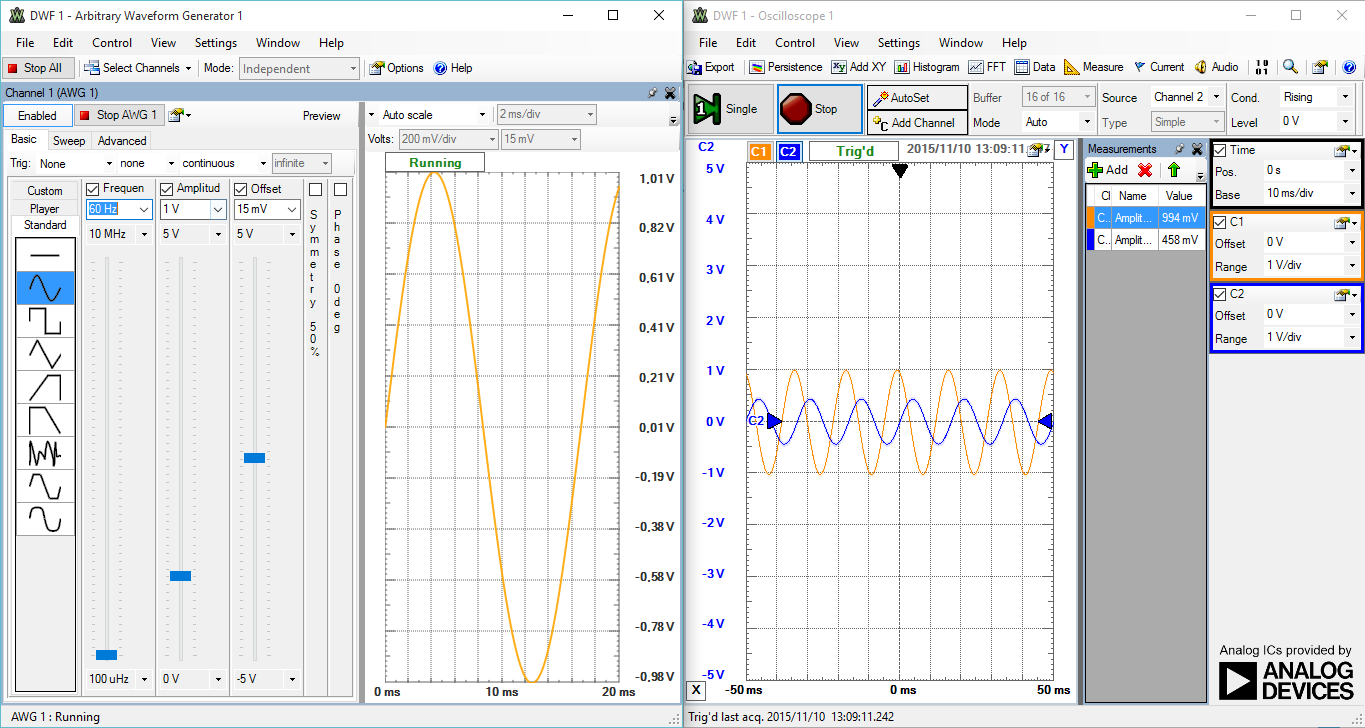
\includegraphics[width=1.0\textwidth]{Figurer/60Hz}
	\caption{Måling for 60 Hz}
	\label{fig:maeling60Hz}
\end{figure}



\section{Software}
\subsection{Design}
I dette beskrives systemets softwaredesign på baggrund af systembeskrivelsen og kravspecifikationen. De overvejelser vi har gjort i forbindelse med design og implementering af software vil blive præsenteret i dette afsnit. 

\subsubsection{Overordnet sekvensdiagram}
Overordnet set ønskes det at udvikle et system, der kan interagerer med en forsker. Diagrammet herunder viser at forskerens opgave består i at starte, tage stilling til nulpunktsjustering og kalibrering samt gemme de ønskede data. Diagrammet er en simpel illustration som viser systemets adfærd gennem alle fem Use Cases. Formålet med dette diagram er udelukkende at skabe et overblik over det samlede system.

\subsubsection{Problemidentifikation}
Første step i software designet er at klarlægge hvilke klasser systemet skal bestå af. Til dette er en domænemodel derfor udarbejdet med udgangspunkt i de fem Use Cases. I de fem Use Cases er de konceptuelle klasser blevet identificeret, og derefter indført som klasser i nedestående domænemodel. Modellen har til formål at vise hvilke dele systemet skal holde styr på. 
Diagrammet viser tydeligt forskerens interaktion med display, samt hvilke handlinger denne interaktion starter i system. Hardware-komponenterne er medtaget for at vise signalets vej fra måleobjekt til system. 

\subsubsection{Klasseidentifikation}
Ud fra domænemodellen kan et klassediagram så udarbejdes, således tager dette diagram også udgangspunkt i de fem Use Cases. Hensigten med et klassediagram er at klarlægge hver klasses individuelle formål. Dermed ses det at denne model er delt op i tre niveauer:
\begin{enumerate}
\item Grænsefladeklasse
\begin{enumerate}
\item Transducer - Indhentet data fra måleobjekt
\item Display - Brugergrænseflade til forsker
\end{enumerate}
\item Kontrolklasse
\begin{enumerate}
\item UC1: Foretag nulpunktsjustering
\item UC2: Foretag kalibrering
\item UC3: Start måling
\item UC4: Gem måling
\item UC5: Afslut måling
\end{enumerate}
\item Domæneklasse
\begin{enumerate}
\item Database
\end{enumerate}
\end{enumerate}

\subsubsection{Metodeidentifikation}
Klasserne i ovenstående klassediagram er med til at definere, hvilke blokke de følgende sekvensdiagrammer må indeholde. Det er yderst vigtigt at der er en sammenhæng mellem klasserne i klassediagrammet og blokkene i sekvensdiagrammet. Vi har valgt at udarbejde et sekvensdiagram for hver enkelt Use Case, hvori systemets interne kommunikation beskrives, når både normalforløb og undtagelser gennemløbes. I alle diagrammerne beskrives forløbet via de metodekald, der er nødvendige for at få de ønskede handlinger mellem blokkene udført. 

\subsection{Implementering}
\subsection{Modultest}
